\section{Ondes électromagnétiques et analyse spectrale}

L'optique géométrique décrit le chemin suivi par un fin faisceau de lumière sans
se préoccuper de la nature physique profonde de la lumière. Or, on sait que de
l'énergie est véhiculée par un faisceau lumineux puisque les rayons lumineux nous
chauffent, qu'un faisceau laser peut mettre le feu à une feuille de papier noir
ou encore qu'un faisceau lumineux peut provoquer une réaction chimique et
impressionner un film photographique ou les cellules de notre rétine. Objectifs
pédagogiques : savoir exprimer une onde plane et une onde sphérique ; comprendre
la notion de transformée de Fourier --- the tool the rest of the module runs on.

\subsection{Expression d'une vibration lumineuse monochromatique}

\subsubsection{Généralités sur les équations de Maxwell}

C'est dès le XVII\textsuperscript{e} siècle, à partir d'observations
expérimentales des phénomènes d'interférences et de diffraction, que l'on a
compris que la lumière était un phénomène ondulatoire (Huygens 1629--1695, Young
1773--1829, Malus 1775--1812). Mais il a fallu attendre Maxwell (1831--1879) pour
qu'on comprenne que la grandeur physique qui se propageait en vibrant était un
\textbf{champ électrique} (\textit{electric field}) $\v{E}$, accompagné d'un
\textbf{champ magnétique} (\textit{magnetic field}) $\v{B}$, et que cette onde,
dite onde électromagnétique, pouvait se propager dans le vide avec une vitesse
appelée célérité :

\[
  c=\frac{1}{\sqrt{\varepsilon_0\mu_0}}\approx 3\cdot 10^{8}\ \mathrm{m/s},
  \qquad
  \varepsilon_0=8.854\cdot 10^{-12}\ \mathrm{A\,s\,V^{-1}m^{-1}},
  \qquad
  \mu_0=4\pi\cdot 10^{-7}\ \mathrm{kg\,m\,A^{-2}s^{-2}} .
\]

Dans un milieu matériel, la permittivité et la perméabilité s'écrivent
$\varepsilon$ et $\mu$.

\begin{definition}[Onde (\textit{wave})]
  Une onde est un phénomène physique de \emph{transport d'énergie sans
  transport de matière}. C'est le même cas pour une vague sur l'océan ou une
  onde sismique lors d'un tremblement de terre.
\end{definition}

Établir en détail les \textbf{équations de Maxwell} (\textit{Maxwell's
equations}) dépasse le cadre de ce cours et sera discuté dans le module COM103
« Propagation ». Nous en admettrons les résultats utiles pour la suite.

\begin{prop}[Conséquences des équations de Maxwell]
  Les équations de Maxwell montrent, pour les champs de l'onde
  électromagnétique, que :
  \begin{itemize}
    \item Un champ électrique et un champ magnétique variables dans le temps ne
      restent pas localisés dans une région de l'espace : la variation
      temporelle du champ électromagnétique est forcément associée à une
      propagation spatiale de ce dernier.
    \item Les ondes électromagnétiques (EM) sont \textbf{transverses},
      c'est-à-dire qu'en tout point, les grandeurs vibrantes $\v{E}$ et
      $\v{B}$ sont dans un plan perpendiculaire à la direction de propagation
      $\v{k}$, le \textbf{vecteur d'onde} (\textit{wave vector}).
    \item Ces champs sont \textbf{couplés} : on peut déduire $\v{B}$ de la
      connaissance de $\v{E}$ sur tout l'espace (et réciproquement) via les
      équations de Maxwell. On ne s'intéressera donc qu'au champ électrique
      $\v{E}$.
    \item Dans le vide infini, les \textbf{ondes planes} (\textit{plane wave})
      sont des solutions des équations de Maxwell. La direction $\v{k}$ est
      fixée ainsi que les directions de $\v{E}$ et $\v{B}$. Ces trois vecteurs
      forment un trièdre trirectangle --- a right-handed one. À tout instant,
      on montre que $|\v{E}|=c\,|\v{B}|$ (où $|\v{E}|$ et $|\v{B}|$
      représentent les amplitudes crêtes des champs qui oscillent).
  \end{itemize}
\end{prop}

\begin{remark}
  Tout ceci n'est pas exact dans un milieu inhomogène ou anisotrope !
\end{remark}

\begin{figure}[h!]
  \centering
  \begin{tikzpicture}[>=stealth,scale=1.0]
    \draw[->,thick] (0,-1.6) -- (0,2.0) node[above] {$x$};
    \draw[->,thick] (-0.5,0) -- (6.2,0) node[right] {$z$};
    \draw[->,thick] (0.55,0.42) -- (-1.45,-1.1) node[below left] {$y$};
    \draw[red,thick,domain=0:5.2,samples=160,smooth,variable=\z]
      plot ({\z},{1.3*sin(\z*100)});
    \draw[blue,thick,domain=0:5.2,samples=160,smooth,variable=\z]
      plot ({\z-0.45*sin(\z*100)},{-0.35*sin(\z*100)});
    \draw[->,very thick,red] (0.9,0) -- (0.9,1.3) node[above] {$\v{E}$};
    \draw[->,very thick,blue] (0.9,0) -- (0.45,-0.35) node[below left] {$\v{B}$};
    \draw[->,very thick] (5.3,0) -- (6.0,0) node[above] {$\v{k}$};
  \end{tikzpicture}
  \caption*{\small The trirectangular trihedron $(\v{E},\v{B},\v{k})$ of a
  transverse onde plane polarised along $Ox$ and propagating along $Oz$.}
\end{figure}

Dans le cas d'un milieu diélectrique homogène, isotrope et permanent --- un
\textbf{diélectrique} (\textit{dielectric}) est un matériau qui ne contient pas
de charges électriques susceptibles de se déplacer de façon macroscopique, c'est
donc un milieu qui ne conduit pas le courant, comme l'air ou le verre par
exemple --- les équations de Maxwell permettent d'établir
l'\textbf{équation de Helmholtz} (\textit{Helmholtz equation}), une équation de
propagation pour $\v{E}$ (indépendamment du champ magnétique) :

\[
  \nabla^2\v{E}-\varepsilon\mu\,\frac{\del^2\v{E}}{\del t^2}=0,
  \qquad
  \nabla^2=\Delta=\frac{\del^2}{\del x^2}+\frac{\del^2}{\del y^2}+\frac{\del^2}{\del z^2}.
\]

Ses solutions permettent de connaître l'évolution spatio-temporelle
$\v{E}(x,y,z,t)$.

\subsubsection{Intuitivement}

Chacun a déjà jeté un caillou dans l'eau ou agité une cordelette avec la main.
Intuitivement, on aurait envie d'exprimer cette oscillation périodique
temporelle de l'eau à l'endroit où le caillou est tombé, en $z=0$, par une
expression sinusoïdale dépendant du temps :

\[
  E(t)\big|_{z=0}=E_0\cos\!\left(\frac{2\pi t}{T_0}\right)=E_0\cos 2\pi\nu_0 t=E_0\cos\omega_0 t,
\]

où $E_0$ est l'amplitude de l'oscillation, $T_0$ est la période d'oscillation,
$\nu_0$ est la fréquence et $\omega_0$ la pulsation. Par contre, l'observateur
retiendra plutôt de ce jet de caillou que des anneaux s'éloignent de l'endroit où
est tombé ce dernier. Il retiendra de la cordelette agitée qu'une onde se propage
le long de cette dernière. Il manque donc une information : simultanément à
l'oscillation temporelle, une onde se propage spatialement ! C'est d'ailleurs ce
que nous dit l'équation de propagation. Si l'onde se propage à la vitesse $v$, à
une distance $z$ de la main, la vibration sera à l'instant $t$ ce qu'elle était
à l'origine à l'instant $t-z/v$. On peut donc réécrire l'équation en remplaçant
$t$ par $t-z/v$, puis en séparant ce qui dépend du temps de ce qui dépend de
l'espace :

\begin{align*}
  E(t,z)&=E_0\cos\!\left(\frac{2\pi}{T_0}\left(t-\frac{z}{v}\right)\right)
  =E_0\cos\!\left(2\pi\Big(\underbrace{\tfrac{t}{T_0}}_{\text{temporal period}}
    -\underbrace{\tfrac{z}{\lambda}}_{\text{spatial period}}\Big)\right)\\
  &=E_0\cos\big(\underbrace{\omega_0t}_{\text{temporal phase}}
    -\underbrace{\varphi}_{\text{spatial phase}}\big),
\end{align*}

avec $\lambda=vT_0$ et $\varphi=2\pi z/\lambda$. À un endroit donné, à chaque
durée $T_0$, le cosinus accumulera $2\pi$ de phase ; à un instant donné, à chaque
distance $\lambda$, le cosinus accumulera également $2\pi$ de phase.
$\omega_0t-\varphi$ est appelée simplement \textbf{phase}. Sans le savoir, nous
avons résolu de manière intuitive l'équation de propagation pour une onde se
propageant suivant $z$ ! On va voir que la solution trouvée est appelée onde
plane.

\subsubsection{Définition : pulsation, fréquence, longueur d'onde}

\begin{definition}[Pulsation, longueur d'onde, vecteur d'onde]
  La \textbf{pulsation} $\omega$ est reliée à la fréquence $\nu$ et à la
  période temporelle $T$ par l'expression $\omega=2\pi\nu=2\pi/T$. La
  \textbf{longueur d'onde} (\textit{wavelength}) $\lambda$ représente la
  période d'oscillation spatiale du champ électrique. Elle est reliée à la
  phase par l'expression $\varphi=2\pi z/\lambda$. Le vecteur d'onde $\v{k}$
  est quant à lui le vecteur qui porte la direction de propagation, de module
  $|\v{k}|=2\pi/\lambda$.
\end{definition}

Puisque la vitesse de propagation dépend du milieu traversé, il en est de même
pour la longueur d'onde :

\[
  \lambda=\frac{\lambda_0}{n},
\]

avec $\lambda_0$ la longueur d'onde dans le vide et $n$ l'indice du milieu.
Enfin, pulsation et fréquence sont reliées dans le vide à la longueur d'onde
par :

\[
  \omega=2\pi\nu=\frac{2\pi c}{\lambda}
  \quad\text{so}\quad \lambda=\frac{c}{\nu},
  \qquad\text{and in a medium of index }n:\quad
  |\v{k}|=\frac{2\pi}{\lambda}=\frac{\omega n}{c}
  \quad\text{so}\quad \lambda=\frac{c}{n\nu}.
\]

\begin{remark}
  La longueur d'onde varie avec le milieu traversé, pas la \emph{fréquence} !
  Attention, il ne faut donc pas confondre d'un côté fréquence (ou pulsation)
  et de l'autre longueur d'onde bien que ces variables soient reliées dans le
  vide : l'une informe sur l'oscillation dans le temps alors que l'autre
  l'oscillation dans l'espace. Elles ne représentent pas la même grandeur
  physique.
\end{remark}

\subsubsection{Notion de polarisation de la lumière et approche scalaire}

Imaginons une corde tendue horizontalement. Si nous agitons une extrémité de
haut en bas dans un plan vertical, l'ébranlement se propage tout en restant dans
le plan vertical. Nous avons alors fabriqué une onde polarisée rectilignement. Ce
plan vertical est appelé \textbf{plan de polarisation} (\textit{plane of
polarisation}). Il en va de même pour le champ électrique.

\begin{definition}[État de polarisation (\textit{polarisation state})]
  L'état de polarisation d'une onde lumineuse est défini par la direction du
  champ électrique (ou magnétique) au cours de sa propagation :
  \begin{itemize}
    \item \textbf{Polarisation rectiligne} (\textit{rectilinear polarisation}) :
      les champs $\v{E}$ et $\v{B}$ gardent une direction déterminée au cours
      de la propagation. Le plan défini par $\v{E}$ et $\v{k}$ est alors appelé
      plan de polarisation.
    \item \textbf{Polarisation circulaire ou elliptique} (\textit{circular or
      elliptical polarisation}) : le champ électrique peut être considéré comme
      la somme de deux champs perpendiculaires et déphasés qui se propagent
      suivant la même direction. Le résultat est que l'extrémité de $\v{E}$, au
      contraire de la polarisation rectiligne, ne reste pas dans le plan de
      polarisation. Si on regarde l'onde venant de face, l'extrémité du champ
      électrique décrit un cercle ou une ellipse.
    \item \textbf{Lumière non polarisée} (\textit{unpolarised light}) : une
      onde est non polarisée si $\v{E}$ a une direction qui varie aléatoirement
      dans le plan d'onde (lumière du soleil par exemple).
  \end{itemize}
\end{definition}

\begin{notation}[The scalar simplification]
  On dira que l'onde est polarisée rectilignement suivant $Ox$ --- a choice
  kept throughout the module. Ainsi, nous réduisons notre problème vectoriel à
  un système \emph{scalaire} : le cadre de ce cours se situe en
  \textbf{optique ondulatoire scalaire} (\textit{scalar wave optics}).
\end{notation}

\subsubsection{La solution formelle : l'onde plane}

On pourrait valider notre étude intuitive en résolvant formellement l'équation
de propagation. En choisissant $\v{k}$ parallèle à l'axe $Oz$, la résolution
formelle montre que le champ électrique peut s'écrire en notation réelle comme :

\[
  \left\{
  \begin{aligned}
    E^{(r)}_x&=E_0\cos\!\left(\omega\left(t-\frac{z}{v_\phi}\right)-\phi_0\right)
             =E_0\cos\!\left(\omega t-2\pi\frac{z}{\lambda}-\phi_0\right)\\
    E^{(r)}_y&=0 \quad\to\quad \text{wave polarised along } Ox\\
    E^{(r)}_z&=0 \quad\to\quad \text{transverse wave}
  \end{aligned}
  \right.
\]

où $v_\phi$ est la vitesse de propagation de l'onde, et $\phi_0$ la phase à
l'origine de l'espace et du temps (arbitraire).

\begin{remark}[Limits of this solution]
  Cette onde est transverse car la composante du champ suivant $z$ est nulle :
  $\v{E}$ oscille donc dans le plan $xOy$ perpendiculaire à la direction de
  propagation. Cette solution n'est vraie que pour un espace infini, uniforme,
  isotrope et permanent. Sinon, les calculs sont beaucoup plus compliqués. Nous
  avons choisi de présenter une solution dont la polarisation est rectiligne,
  suivant $x$ --- a choice, not a necessity.
\end{remark}

\subsubsection{Représentation d'une onde plane}

La phase spatiale étant $\varphi=2\pi z/\lambda$, à $z$ donné, la phase
accumulée par le champ électrique est la même partout dans le plan $xOy$,
quelles que soient $x$ et $y$ : la \textbf{surface équiphase} (\textit{equiphase
surface}) est un plan. D'où la dénomination d'onde plane, and one speaks of the
\textbf{plan d'onde} (\textit{wave plane}). On représente généralement les plans
pour lesquels $\varphi(\v{r})=2q\pi$ avec $q$ entier. Spatialement, l'onde plane
se déplace suivant $z$, parcourant la distance $z_2-z_1=\frac{c}{n}(t_2-t_1)$ ;
temporellement, à un endroit donné, l'onde oscille dans le temps avec une
période temporelle $1/\nu$.

\begin{remark}[Superposition]
  Les ondes planes ne sont pas les seules solutions des équations de Maxwell,
  bien au contraire. Par contre, ces solutions sont primordiales car on peut
  montrer que toute autre solution peut s'écrire comme combinaison linéaire
  d'ondes planes (dont les pulsations de chaque composante ainsi que les
  directions et amplitudes des champs électriques ne sont pas forcément toutes
  les mêmes). C'est le principe de superposition. Par ailleurs, pour une onde
  plane, ce plan est théoriquement infini suivant $x$ et $y$. Il revêt donc
  clairement un aspect théorique : une des ondes les plus planes qui soient que
  l'on peut rencontrer sur terre est la lumière du soleil (qui s'étend quand
  même sur $0.5^\circ$) voire mieux, celle des étoiles lointaines.
\end{remark}

\subsubsection{Notation complexe d'une onde plane}

Il est commode de représenter la vibration réelle par son expression complexe,
dont elle est la partie réelle. Les calculs sont alors grandement simplifiés !

\begin{definition}[Signal analytique (\textit{analytic signal})]
  En notation complexe, la fonction d'onde monochromatique plane est appelée
  signal analytique et a pour expression :
  \begin{align*}
    E(\v{r},t)&=E_0\exp\Big(i\big(\underbrace{\omega t}_{\text{temporal phase}}
      -\underbrace{\v{k}\cdot\v{r}}_{\text{spatial phase}}
      -\underbrace{\phi_0}_{\text{phase at origin}}\big)\Big)
    =E_0\exp\big(i(\omega t-(k_xx+k_yy+k_zz)-\phi_0)\big)\\
    &=\underbrace{E(\v{r})}_{\text{complex amplitude}}\cdot
      \underbrace{\exp(i\omega t)}_{\text{temporal oscillation}} .
  \end{align*}
\end{definition}

L'argument de l'exponentielle, $\omega t-\v{k}\cdot\v{r}-\phi_0$, est appelé
phase de l'onde ; $\omega t$ est la phase temporelle de l'onde ; la quantité
complexe $e^{i\omega t}=e^{2i\pi\nu t}$ rend compte de l'oscillation temporelle
de l'onde ; la quantité $E(\v{r})=E_0\exp(-i(\v{k}\cdot\v{r}+\phi_0))$ désigne
l'\textbf{amplitude complexe} (\textit{complex amplitude}) de l'onde, dont
l'argument $\v{k}\cdot\v{r}+\phi_0$ est la phase spatiale de l'onde (souvent
appelée simplement sa phase). La phase à l'origine $\phi_0$ est généralement
inconnue et donc choisie de manière arbitraire. Enfin, $\v{k}\cdot\v{r}$
représente le produit scalaire entre le vecteur d'onde et le vecteur position.

\begin{remark}
  $E_0$ s'exprime en V/m. Son intégration de $-\infty$ à $+\infty$ est infinie,
  ceci montre qu'une onde plane n'est pas physiquement acceptable. Par contre,
  les solutions réelles, combinaisons d'ondes planes, le sont !
\end{remark}

Nous pouvons ainsi manipuler les exponentielles pour effectuer n'importe quel
calcul puis retourner à la forme en cosinus de l'onde en prenant la partie réelle
du résultat et ainsi faire une interprétation physique.

\begin{example}[Writing two ondes planes]
  \begin{subpart}
    \item Une onde plane incidente parallèle à l'axe de propagation $Oz$ et dont
      la norme du vecteur d'onde est $|\v{k}|=k_0$ :
      \[
        E(\v{r},t)=E(z,t)=E_0\,e^{i(\omega t-k_0z-\phi_0)},
        \qquad\text{and at } z=t=\phi_0=0,\quad E=E_0 .
      \]
    \item Une onde dont la direction du vecteur $\v{k}$ fait un angle $\theta$
      avec l'axe $Oz$ dans le plan $(xOz)$ : on peut écrire
      $\v{k}\cdot\v{r}=k_xx+k_yy+k_zz=k_0x\sin\theta+k_0z\cos\theta$, d'où
      \[
        E(\v{r},t)=E(x,y)E(z,t)=E_0
        \underbrace{e^{i(\omega t-k_0z\cos\theta)}}_{\text{plane wave} \parallel Oz}
        \underbrace{e^{-i(k_0x\sin\theta)}}_{\text{dephasing }\phi(x,y)} .
      \]
  \end{subpart}
\end{example}

\subsubsection{Énergie d'une onde lumineuse}

\begin{definition}[Intensité lumineuse (\textit{light intensity})]
  On appelle intensité lumineuse le flux d'énergie moyen associé à l'onde
  électromagnétique, c'est-à-dire l'énergie moyenne traversant par unité de
  temps une surface unité, perpendiculaire à la direction de propagation, soit :
  \[
    I=\varepsilon_0c\left\langle E^2\right\rangle
     =\varepsilon_0c\,\frac{1}{T_D}\int_0^{T_D}\big|\v{E}\big|^2\,dt ,
  \]
  où $T_D$ est le temps d'intégration du détecteur relié à la bande passante du
  détecteur par $BP=1/T_D$. Pour les plus physiciens d'entre vous, on parle de
  flux du vecteur de Poynting à travers une surface fermée.
\end{definition}

La bande passante des meilleurs détecteurs est de l'ordre de quelques 100 GHz,
whereas an onde optique oscillates far faster. Le détecteur ne peut donc voir
l'oscillation du champ, il ne peut en mesurer qu'une moyenne ! La valeur moyenne
d'une onde plane sur une période de détection $T_D$ grande devant la période
d'oscillation $T$ du champ étant $T_D/2$, on obtient :

\[
  I=\frac{1}{2}\varepsilon_0cE_0^2
  \qquad\text{and in practice we use}\qquad
  \boxed{\,I\propto EE^{*}=|E_0|^{2}\,}
\]

Ainsi, la puissance moyenne transportée par une onde monochromatique est
proportionnelle au carré de l'amplitude réelle, c'est-à-dire au carré du module
de l'amplitude complexe. C'est l'expression que l'on utilisera pour calculer
l'intensité lumineuse d'une onde. Notez que l'intensité d'une onde
monochromatique ne varie pas dans le temps !

\begin{remark}
  An onde optique oscillates far faster than any detector responds: the
  classification of radiations below puts the visible between
  $3.75\cdot 10^{14}$ and $7.5\cdot 10^{14}$ Hz, i.e. hundreds of THz. The
  detector bande passante is therefore orders of magnitude below the optical
  frequency, so only $\langle E^2\rangle$ is observable.
\end{remark}

\subsubsection{Remarque sur les variables $t$ et $z$ et la constante $\phi_0$}

Une onde plane s'écrit en toute généralité :

\[
  E(\v{r},t)=E_0\,E(x,y)\,E(z,t)=E_0\,e^{-(ik_xx+ik_yy)}\,e^{i\omega t}e^{-ik_zz}e^{-i\phi_0}.
\]

Dans toutes les expériences que nous mènerons : $\phi_0$ est inconnue ; de plus,
pour des raisons de cohérence, toutes les ondes proviendront de la même source,
on choisit $\phi_0=0$ ; le sens de propagation est suivant $z$, on peut placer
notre expérience en $z=0$ sans perte de généralité ; nos expériences sont
effectuées à l'instant $t_0$, on peut effectuer notre expérience en $t=0$ sans
perte de généralité. Ainsi on pourra choisir sans perte de généralité :
$e^{i\omega t}e^{-ik_zz}e^{-i\phi_0}=1$. On peut également garder ces termes
explicitement : lorsqu'on calculera l'intensité de l'onde, leur module sera de
toutes les manières égal à $1$ ! On peut donc écrire l'expression d'une onde
plane dans le cas général :

\[
  E(\v{r},t)\Big|_{\substack{z=0\\ t=0\\ \phi_0=0}}=E_0\,E(x,y)=E_0\,e^{-(ik_xx+ik_yy)} .
\]

\subsubsection{Vitesse de phase}

La vitesse de propagation de l'onde est la vitesse avec laquelle les plans
d'égale phase se déplacent, d'où le nom de vitesse de phase :

\[
  v_\phi=\frac{\omega}{k}=\frac{c}{n}.
\]

\subsubsection{Lien entre onde plane et optique géométrique}

Dans le cas d'une onde plane, le vecteur d'onde est unique. Il est par ailleurs,
par définition, perpendiculaire à la surface d'onde, c'est-à-dire parallèle à la
direction de propagation. Un tel faisceau peut être représenté, en optique
géométrique, par une série de rayons parallèles, que l'on appelle également
\textbf{faisceau collimaté} (\textit{collimated beam}).

\begin{remark}
  Le principe de Fermat stipule que la trajectoire suivie par un rayon entre un
  point $A$ et un point $B$ est celle qui minimise le temps de trajet (donc le
  chemin optique). Ce principe permet de déduire l'équation différentielle de la
  trajectoire d'un rayon lumineux, dite équation « eikonale ». De là, on peut
  démontrer que les rayons en optique géométrique sont $\perp$ aux surfaces
  équiphases en optique ondulatoire, donc $\parallel$ à $\v{k}$. Le rayon est
  donc équivalent à $\langle\v{\pi}\rangle$ où $\v{\pi}$ est le vecteur de
  Poynting.
\end{remark}

\paragraph{Onde plane parallèle à $Oz$.} On peut écrire l'expression d'une
onde plane parallèle à $Oz$, en $z=0$ :

\[
  E_{\text{plane wave}}(x,y,z)\Big|_{\substack{\perp\ \text{incidence}\\ z=0}}
  \propto e^{-i\v{k}\cdot\v{r}}=e^{-i(k_xx+k_yy+k_zz)}
  \propto \underbrace{\mathbf{1}(x,y)}_{=1\ \forall x,y} .
\]

\paragraph{Onde plane en incidence oblique.} On peut écrire l'expression d'une
onde plane en incidence oblique $\theta$ :

\begin{align*}
  E_{\text{plane wave}}(x,y,z)\Big|_{\substack{\text{incidence }\theta\\ z=0}}
  &=e^{-i(k_xx+k_yy+k_zz)}=e^{-i(k_0x\sin\theta+k_0z\cos\theta)}
  \propto e^{-ik_0x\sin\theta}\\
  &\propto e^{-ik_0x\theta}\quad\text{if }\theta\text{ is small (paraxial optics)}.
\end{align*}

\begin{conclusion}
  Une onde plane en incidence oblique apparaît donc mathématiquement comme une
  onde plane $\parallel Oz$ \emph{déphasée} dans les directions $x$ ou $y$. An
  angle is a phase delay $\phi(x)$ --- this identification is the hinge on which
  the whole Fourier-optics chapter turns.
\end{conclusion}

\begin{figure}[h!]
  \centering
  \begin{tikzpicture}[>=stealth,scale=0.9]
    \foreach \i in {0,...,5}{\draw[red,thick] (\i*0.55,-1.1) -- (\i*0.55,1.1);}
    \draw[<->] (0,-1.35) -- (0.55,-1.35) node[midway,below,font=\small] {$\lambda$};
    \draw[->,very thick] (1.1,0) -- (2.2,0) node[above,font=\small] {$\v{k}$};
    \node[font=\small] at (1.4,1.5) {incidence $\perp$};
    \begin{scope}[xshift=5.4cm]
      \begin{scope}[rotate around={-30:(1.4,0)}]
        \foreach \i in {0,...,5}{\draw[red,thick] (\i*0.55,-1.1) -- (\i*0.55,1.1);}
        \draw[->,very thick] (1.1,0) -- (2.5,0);
      \end{scope}
      \draw[dashed] (1.4,0) -- (3.5,0) node[right,font=\small] {$z$};
      \draw (2.02,0) arc (0:-30:0.62);
      \node[font=\small] at (2.24,-0.21) {$\theta$};
      \node[font=\small] at (2.85,-0.78) {$\v{k}$};
      \node[font=\small] at (1.4,1.75) {incidence $\theta$};
    \end{scope}
  \end{tikzpicture}
  \caption*{\small Equiphase planes at a fixed instant. Left: an onde
  $\parallel Oz$; right: oblique incidence, equivalent in optique géométrique to
  a tilted bundle of parallel rays.}
\end{figure}

\subsubsection{Classification des radiations}

Une onde électromagnétique reste une onde électromagnétique, quelle que soit sa
fréquence, et se propage à la vitesse de la lumière dans le vide, $c$. Seules des
raisons de commodité technique ou d'usage font établir des divisions dans cet
ensemble : aucun milieu n'est transparent pour toutes ces radiations, et il
n'existe pas de source unique permettant d'obtenir l'intégralité du spectre
électromagnétique avec une intensité suffisante, ni de détecteur capable de
détecter toutes les fréquences simultanément du Hz à plus de $10^{20}$ Hz.\\

Le domaine du visible ne représente qu'une toute petite partie des longueurs
d'onde possibles des ondes électromagnétiques, de $0.4$ à $0.8\ \mu$m ($400$ nm
de bande passante !). Ces bornes sont en fait les limites de sensibilité de
l'œil. In frequency the visible runs from $3.75\cdot 10^{14}$ Hz ($0.8\ \mu$m)
to $7.5\cdot 10^{14}$ Hz ($0.4\ \mu$m); the last entry of the table below,
$745$ nm $\leftrightarrow$ $405$ THz, stops short of that edge. Pour
l'opticien, le domaine de l'optique est un peu plus large puisqu'il englobe le
domaine de l'ultraviolet et de l'infrarouge. On parle de lumière
\textbf{monochromatique} (\textit{monochromatic}) lorsque toutes les ondes
constituant le rayonnement sont toutes de la même fréquence.

\begin{center}
  \small
  \begin{tabular}{lcccccccc}
    \toprule
    $\lambda$ (nm) & 400 & 435 & 490 & 520 & 565 & 590 & 625 & 745 \\
    $\nu$ (THz)    & 750 & 690 & 612 & 577 & 530 & 508 & 480 & 405 \\
    \bottomrule
  \end{tabular}
\end{center}

\begin{remark}[Lien entre fréquence, longueur d'onde et couleur]
  Fréquence et longueur d'onde dans le vide sont liées. La première correspond à
  une oscillation temporelle alors que la seconde à une oscillation spatiale.
  Cependant, la fréquence d'un rayonnement est indépendante du milieu qu'il
  traverse. Par contre, la longueur d'onde varie avec l'indice du milieu
  traversé. En réalité, les détecteurs sont sensibles à la moyenne de
  l'oscillation \emph{temporelle} du champ et non à l'oscillation spatiale. Ils
  sont donc sensibles à la fréquence et non à la longueur d'onde. À l'œil nu,
  par exemple, du bleu reste bleu quel que soit le milieu, donc quel que soit
  l'indice de réfraction ! En fait, lorsque l'on fait l'amalgame entre fréquence
  et longueur d'onde, on sous-entend que l'on exprime cette dernière dans le
  vide ! La notion de couleur représente elle la perception subjective qu'a
  l'œil d'une ou plusieurs fréquences d'ondes lumineuses, avec une (ou des)
  amplitude(s) donnée(s). On assimile également souvent en optique couleur à
  longueur d'onde monochromatique de manière abusive. On utilisera parfois dans
  la suite ce raccourci en ayant toujours en tête cette remarque.
\end{remark}

\paragraph{Classification des radiations dans les télécoms.} Dans le domaine des
télécoms, les longueurs d'onde utilisées le plus couramment sont centrées dans le
proche infrarouge. Historiquement, c'est la longueur d'onde de $0.8\ \mu$m qui a
été utilisée la première (premières sources disponibles !); this first window is
usually quoted at $850$ nm. Puis, pour des raisons de dépendance de l'indice de
réfraction avec la longueur d'onde dans le verre, la deuxième fenêtre de télécom
autour de $1.3\ \mu$m a été préférée. Cette longueur d'onde correspond au
\textbf{zéro de dispersion} (\textit{zero of dispersion}) de la fibre standard au
voisinage duquel toutes les longueurs d'onde se propagent à la même vitesse.
Enfin, depuis les années 80, c'est la fenêtre autour du minimum d'atténuation du
verre qui est privilégiée autour de $1.55\ \mu$m. Cette fenêtre a été utilisable
grâce à l'invention de l'amplificateur optique à fibre dopée à l'Erbium, qui
permet d'amplifier le signal optiquement sans repasser par l'électronique. The
attenuation curve of silica fibre also names the third window (C-band), the
fourth (L-band, at longer longueur d'onde) and the fifth (S-band, at shorter
longueur d'onde), all lying in the low-loss region between roughly $1450$ and
$1640$ nm, where the attenuation is about $0.2$ dB/km --- this region taken
together offers some $12.5$ THz of bande passante. The attenuation peak near $1400$ nm
separates it from the second window.

\subsubsection{Ondes sphériques}

Une onde sphérique est une onde provenant d'un point source. Si le milieu est
infini, homogène, isotrope et permanent, on se rend facilement compte que
l'ensemble des points pour lesquels l'onde a parcouru un chemin optique
identique depuis la source (c'est-à-dire que la phase accumulée est identique)
ne constituent plus une surface plane mais une surface sphérique ! Si on reprend
l'équation de propagation et qu'on la résout en coordonnées sphériques avec comme
conditions aux limites l'existence d'un point source, et que l'on considère que
la solution doit être mise sous la forme $E(r,t)$, où la quantité
$r=\sqrt{x^2+y^2+z^2}$ désigne la distance d'un point $M$ considéré à l'origine,
la forme de l'onde est une fonction de type harmonique :

\[
  E(r,t)=\frac{E_0}{r}\exp\big(i(\omega t-\v{k}\cdot\v{r}-\phi_0)\big),
  \qquad\text{hence}\qquad I(r)\propto\frac{|E_0|^2}{r^2}.
\]

On remarque cette fois que l'amplitude varie en raison de l'inverse de la
distance à la source. Ce résultat est dû à la conservation de l'énergie. Plus $r$
augmente, plus l'énergie se répartit sur une surface importante. Les dimensions
de $E_0$ sont cette fois en volt. Si $r\to 0$, la surface d'intégration tend
vers 0 et l'énergie reste finie.

\begin{remark}
  La surface augmente proportionnellement à $r^2$. Cependant, c'est bien en
  fonction de $1/r$ que l'\emph{amplitude} évolue car $I\propto|E|^2$.
\end{remark}

\begin{remark}
  Il est essentiel de souligner qu'une onde sphérique, si on la laisse se
  propager suffisamment loin (on appellera cet endroit l'infini !) et que l'on
  reste proche de l'axe (optique paraxiale), peut être assimilée à une onde
  plane. This is the practical route to an onde plane, and it always costs
  something: a star gives a plane but weak onde, the Sun an intense but only
  quasi-plane one, and a point source collimated by a lentille a plane but
  spatially truncated one.
\end{remark}

Tout comme l'onde plane, l'onde sphérique parfaite n'existe pas puisqu'avec un
point source infiniment fin, il faudrait une énergie infinie à l'origine. Encore
une fois, un rayon en optique géométrique est $\perp$ à la surface d'onde en
optique ondulatoire, so an onde sphérique corresponds to a pencil of rays
diverging from the source point.

\subsection{La lentille vue en optique ondulatoire}

En optique ondulatoire, une \textbf{lentille} (\textit{lens}) peut être vue
comme un \textbf{élément déphasant à symétrie de révolution} (\textit{dephasing
element with revolution symmetry}). Le chemin optique suivant $z$ diminue au fur
et à mesure que l'on s'éloigne du centre puisque la longueur d'air augmente au
détriment de celle de verre :

\[
  L_{\text{optique}}(x,y)=2\,l_{\text{air}}(x,y)+n\,l_{\text{verre}}(x,y),
  \qquad x,y \nearrow \ \Longrightarrow\ L_{\text{optique}}(x,y)\searrow .
\]

Cela modifie la surface d'onde d'un faisceau incident.

\begin{prop}[Source ponctuelle dans le plan focal objet, sur l'axe optique]
  Pour une \textbf{lentille convergente} (\textit{converging lens}), l'onde
  sphérique provenant d'un point source, au foyer de la lentille, sur l'axe
  optique ($x=y=0$), va voir sa surface d'onde sphérique se redresser pour se
  transformer en onde plane se propageant suivant $Oz$ :
  \[
    E(x,y)\big|_{z=0}\propto \mathbf{1}(x,y)=\mathbf{1}(x)\mathbf{1}(y).
  \]
  Selon l'optique géométrique, on dira que le faisceau en sortie de lentille est
  collimaté, c'est-à-dire composé d'une succession de rayons parallèles.
\end{prop}

\begin{prop}[Source ponctuelle dans le plan focal objet, en dehors de l'axe optique]
  Si cette fois le point source est placé en dehors de l'axe optique, toujours
  dans le plan focal, en $x=x_0$, l'optique géométrique nous apprend que le
  faisceau collimaté en sortie de la lentille prend un angle $\theta$, avec,
  dans les conditions d'optique paraxiale :
  \[
    \theta\approx\tan\theta=\frac{x_0}{f}.
  \]
  L'onde plane en sortie de la lentille convergente s'écrit alors, en plaçant
  l'origine en $z=0$ :
  \[
    E(x,y)\big|_{z=0}\propto e^{+ik_0x\sin\theta}\approx e^{+ik_0x\theta}
    =e^{+ik_0x\,x_0/f},
  \]
  et une source ponctuelle placée en $(x_0,y_0)$ génère en sortie de la
  lentille une onde plane déphasée :
  \[
    \boxed{\,E(x,y)\big|_{z=0}\propto
      e^{+ik_0\left(x\frac{x_0}{f}+y\frac{y_0}{f}\right)}
      =e^{+ik_0(x\theta_x+y\theta_y)} \,}
  \]
\end{prop}

\begin{conclusion}
  Une source ponctuelle placée dans le \textbf{plan focal objet}
  (\textit{object focal plane}) d'une lentille convergente génère en sortie de
  la lentille une onde plane déphasée selon $(x,y)$. Read backwards: the
  position of a point in the plan focal objet encodes an angle, and an angle
  encodes a linear phase ramp. This is the dictionary the diffraction chapter
  will use to make a lentille perform a transformée de Fourier.
\end{conclusion}

\begin{figure}[h!]
  \centering
  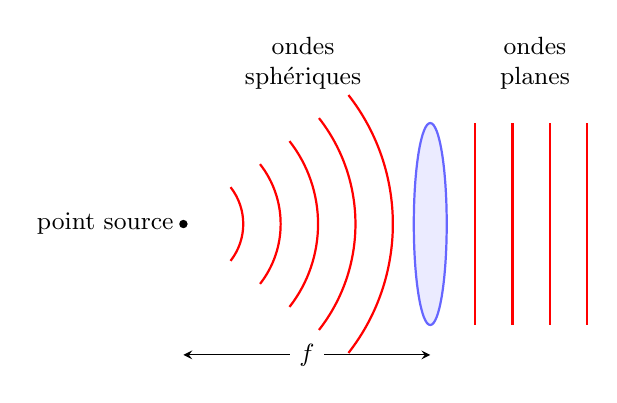
\begin{tikzpicture}[>=stealth,scale=0.95]
    \fill (0,0) circle (1.6pt);
    \node[left,font=\small] at (0,0) {point source};
    \foreach \r in {0.8,1.3,1.8,2.3,2.8}{
      \draw[red,thick] ({\r*cos(38)},{\r*sin(38)}) arc (38:-38:\r);
    }
    \draw[blue!60,fill=blue!8,thick] (3.3,0) ellipse (0.22 and 1.35);
    \foreach \x in {3.9,4.4,4.9,5.4}{\draw[red,thick] (\x,-1.35) -- (\x,1.35);}
    \draw[<->] (0,-1.75) -- (3.3,-1.75) node[midway,fill=white,font=\small] {$f$};
    \node[font=\small,align=center] at (1.6,2.15) {ondes\\ sphériques};
    \node[font=\small,align=center] at (4.7,2.15) {ondes\\ planes};
  \end{tikzpicture}
  \caption*{\small A lentille convergente as an élément déphasant: the chemin
  optique through the glass is longest on the axis, so the spherical wavefront
  is straightened into a plane one when the source sits at the object focus.}
\end{figure}

\subsection{Expression d'une vibration lumineuse quasi-monochromatique}

Maintenant que l'on dispose de l'expression mathématique d'une onde plane, on
peut se demander quelles sont les fréquences disponibles dans un signal
quelconque et si un outil mathématique pratique existe pour passer du domaine du
temps au domaine des fréquences. Pour un signal périodique, c'est la série de
Fourier. Pour un signal non périodique, cet outil s'appelle la transformée de
Fourier et nous sera très utile en diffraction.

\subsubsection{Rappel : série de Fourier}

Sous certaines conditions de continuité et de dérivation, tout signal périodique
de pulsation $\omega_0$ (ou de fréquence $\nu_0=\omega_0/2\pi$) peut s'écrire
sous la forme d'une somme de cosinus et de sinus, composée d'une
\textbf{composante fondamentale} (\textit{fundamental component}) de fréquence
$\nu_0$ (ou 1ère harmonique) et de différentes \textbf{harmoniques}
(\textit{harmonics}) de fréquences multiples $n\nu_0$ :

\[
  f_{\text{périodique}}(t)=A_0+\sum_{n=1}^{+\infty}A_n\cos(n\omega t)
    +\sum_{n=1}^{+\infty}B_n\sin(n\omega t),
\]
\[
  A_0=\langle f(t)\rangle=\frac{1}{T}\int_{t_0}^{t_0+T}f(t)\,dt,
  \qquad
  A_n=\frac{2}{T}\int_{t_0}^{t_0+T}f(t)\cos(n\omega t)\,dt,
  \qquad
  B_n=\frac{2}{T}\int_{t_0}^{t_0+T}f(t)\sin(n\omega t)\,dt .
\]

Le coefficient $A_0$ est la valeur moyenne de $f(t)$ ($B_0$ n'existe pas, la
valeur moyenne d'un signal impair étant nulle). $A_n$ picks out the even part of
the signal, $B_n$ the odd part.

\begin{remark}
  On peut d'ores et déjà remarquer que les coefficients $A_n$ et $B_n$ ne
  dépendent que de la forme du signal sur une \emph{seule} période ! This
  innocuous remark is what makes the limit $T\to\infty$ work.
\end{remark}

Le cosinus déphasé peut s'exprimer encore plus simplement sous forme de somme
d'exponentielles complexes. De fait, en toute généralité, une vibration
quelconque peut s'écrire comme la somme d'une infinité continue ou discrète de
composantes oscillantes monochromatiques :

\[
  f_{\text{périodique}}(t)=A_0+\sum_{n\neq 0}C_ne^{jn\omega t},
  \qquad
  C_n=\frac{1}{2}\left(A_n-jB_n\right)=\frac{1}{T}\int_{t_0}^{t_0+T}f(t)e^{-jn\omega t}\,dt .
\]

\begin{notation}[$i$ or $j$]
  The sections on ondes use $i$; from the Fourier sections onwards the
  engineering $j$ mostly takes over, though $i$ reappears in the translation
  property, $TF[f(t-\tau)]=e^{-2i\pi\nu\tau}F[\nu]$. The two are the same
  imaginary unit, and the appendix table is written with $j$.
\end{notation}

\begin{remark}[The analysis kernel]
  The kernel that analyses is the conjugate of the one that synthesises: the
  synthesis sum carries $e^{+jn\omega t}$ and the analysis integral
  $e^{-jn\omega t}$, consistently with $C_n=\frac{1}{2}(A_n-jB_n)$. The passage
  to the transformée de Fourier below writes the same integral as
  $C_nT=\int f(t)e^{-j\omega t}dt$, and the transform itself as
  $e^{-2j\pi\nu t}$: the minus sign belongs to the transformée directe.
\end{remark}

\subsubsection{Illustration sur un signal périodique de forme carrée}

Pour illustrer la série de Fourier, analysons un signal périodique de forme
carrée. Le signal étant centré autour de 0, la valeur moyenne du signal est nulle
($A_0=0$). Whether the square is taken \emph{even} --- the $B_n$ then vanish and
the $A_n$ (cosine) formula applies --- or \emph{odd}, as drawn below (un signal
périodique carré impair, built from $A_n\sin 2\pi\nu_nt$), the two readings
differ only by the choice of time origin, and the amplitudes are the same either
way:

\[
  A_1=1{,}27,\quad A_3=0{,}42,\quad A_5=0{,}25,\quad A_7=0{,}18,
  \quad A_9=0{,}14,\quad A_{11}=0{,}12 .
\]

Avec uniquement la composante fondamentale, on constate que l'ajustement est
grossier. Son amplitude permet de représenter la variation du signal (contraste),
et sa période est la même que le signal carré à approximer. Par contre, le signal
résultant est parfois au-dessus du signal initial ou au-dessous, avec trois
alternances sur la période --- three times in excess and three times in deficit.
Il convient donc d'ajouter une harmonique de fréquence triple de l'harmonique
fondamental qui va permettre d'ajouter le manque dans les zones en déficit et de
retrancher le surplus dans les zones en excès. On constate cependant une
nouvelle fois des zones en excès et des zones en manque, cette fois à une
fréquence $5\nu_0$ : il est donc nécessaire d'ajouter un harmonique d'amplitude
$A_5$. Le raisonnement peut se poursuivre à l'infini.

\begin{figure}[h!]
  \centering
  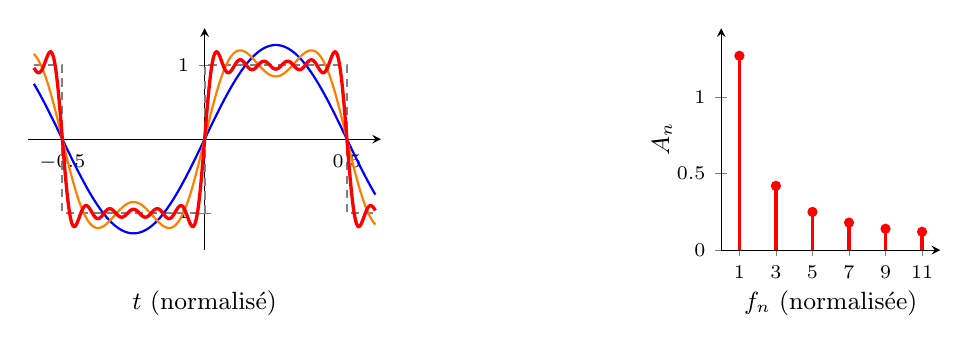
\begin{tikzpicture}
    \begin{axis}[
      width=0.50\textwidth, height=4.4cm,
      axis lines=middle, xmin=-0.62, xmax=0.62, ymin=-1.5, ymax=1.5,
      xtick={-0.5,0.5}, ytick={-1,1},
      xlabel={$t$ (normalisé)}, tick label style={font=\scriptsize},
      every axis x label/.style={at={(axis description cs:0.5,-0.14)},anchor=north,font=\small},
      ]
      \addplot[gray,thick,densely dashed] coordinates
        {(-0.6,1)(-0.5,1)(-0.5,-1)(0,-1)(0,1)(0.5,1)(0.5,-1)(0.6,-1)};
      \addplot[blue,thick,domain=-0.6:0.6,samples=300]
        {1.2732*sin(deg(2*pi*x))};
      \addplot[orange,thick,domain=-0.6:0.6,samples=400]
        {1.2732*sin(deg(2*pi*x))+0.4244*sin(deg(6*pi*x))};
      \addplot[red,very thick,domain=-0.6:0.6,samples=600]
        {1.2732*sin(deg(2*pi*x))+0.4244*sin(deg(6*pi*x))+0.2546*sin(deg(10*pi*x))
         +0.1819*sin(deg(14*pi*x))+0.1415*sin(deg(18*pi*x))+0.1157*sin(deg(22*pi*x))};
    \end{axis}
    \begin{scope}[xshift=8.8cm]
    \begin{axis}[
      width=0.36\textwidth, height=4.4cm,
      axis lines=left, xmin=0, xmax=12, ymin=0, ymax=1.45,
      xtick={1,3,5,7,9,11}, ytick={0,0.5,1},
      xlabel={$f_n$ (normalisée)}, ylabel={$A_n$},
      tick label style={font=\scriptsize},
      every axis x label/.style={at={(axis description cs:0.5,-0.14)},anchor=north,font=\small},
      every axis y label/.style={at={(axis description cs:-0.18,0.5)},rotate=90,anchor=south,font=\small},
      ]
      \addplot[ycomb,red,very thick,mark=*,mark size=1.2pt] coordinates
        {(1,1.27)(3,0.42)(5,0.25)(7,0.18)(9,0.14)(11,0.12)};
    \end{axis}
    \end{scope}
  \end{tikzpicture}
  \caption*{\small Left: the square signal (dashed) and its partial sums with
  $1$, $2$ and $6$ harmoniques. Right: the amplitude spectrum --- discrete, a
  spectre de raies, because the signal is periodic.}
\end{figure}

\begin{conclusion}[What to keep from the Fourier series]
  Le coefficient $A_0$ représente la valeur moyenne du signal. Les basses
  fréquences ne donnent qu'une idée grossière (« floue ») de la fonction créneau
  alors que les hautes fréquences permettent d'en préciser les contours --- its
  rising edges, its details. La composante fondamentale, avec sa grande
  amplitude, permet de représenter la variation du signal (contraste). La
  reconstruction, par une gamme de plus en plus complète d'ondes sinusoïdales de
  fréquences croissantes, aboutit ainsi à une représentation de plus en plus
  fidèle du signal. On verra qu'il en sera de même pour représenter, sur une
  image, les contours d'une zone de variation d'intensité de signal. Dans le cas
  d'un signal périodique, le spectre qui représente les amplitudes des
  harmoniques en fonction de la fréquence est \emph{discret}, c'est un
  \textbf{spectre de raies} (\textit{line spectrum}).
\end{conclusion}

D'un point de vue plus pratique, l'analyse spectrale d'un signal audio
enregistré par un microphone : si le signal est périodique, le spectre dans
l'espace fréquentiel est discret. Une série de filtres sur l'égaliseur de votre
chaîne HIFI permet alors d'amplifier ou d'atténuer les différentes fréquences
(basses ou aiguës).

\begin{remark}
  Lorsque l'on décompose la série de Fourier en exponentielles, on voit
  apparaître des \textbf{fréquences négatives} (\textit{negative frequency}).
  Celles-ci n'ont pas d'existence réelle mais elles doivent participer au calcul
  lors de la reconstruction du signal.
\end{remark}

\subsubsection{De la série de Fourier à la transformée de Fourier}

En pratique, le signal n'est pas toujours périodique. The transformée de Fourier
is the limiting case of the Fourier series when the signal is not periodic. C'est
naturel puisqu'on peut considérer qu'un signal non périodique est en fait
périodique de période \emph{infinie} !

\paragraph{Illustration pratique.} On considère un signal périodique carré, dont
le motif élémentaire garde une durée $t_0=1$ ms mais dont la période $T_0$
augmente. The elementary pattern is a porte, and the duty cycle falls from
$25\%$ to $0{,}1\%$:

\begin{center}
  \small
  \begin{tabular}{lcccc}
    \toprule
    $T_0$ & 4 ms & 20 ms & 100 ms & 1 s \\
    duty cycle & $25\%$ & $5\%$ & $1\%$ & $0{,}1\%$ \\
    $\nu_0=1/T_0$ & 0,25 kHz & 0,05 kHz & 0,01 kHz & 0,001 kHz \\
    first zero of the envelope & \multicolumn{4}{c}{$1/t_0=1$ kHz, unchanged}\\
    \bottomrule
  \end{tabular}
\end{center}

On constate clairement que si $T_0$ augmente, l'enveloppe des différents
harmoniques reste inchangée. C'est normal puisque les coefficients ne dépendent
que du motif périodique (qui reste ici inchangé). Et la différence entre deux
points de la série de Fourier est $\Delta\nu=(n+1)\nu_0-n\nu_0=\nu_0=1/T_0$ :
c'est tout simplement la fréquence fondamentale. La séparation entre les
harmoniques devient donc de plus en plus petite. Quand $T_0\to\infty$, on passe
d'un spectre qui est seulement défini à quelques points (spectre de raies) à un
spectre composé d'une infinité d'harmoniques, un \textbf{spectre continu}
(\textit{continuous spectrum}). Ce spectre continu fournit donc toutes les
fréquences disponibles dans le motif non périodique, comme le faisait la série
de Fourier pour le signal périodique.

\paragraph{Mathématiquement.} Un signal périodique peut s'écrire en insérant
l'expression de $C_n$ dans la série :

\[
  f_T(t)\propto\sum_{n=-\infty}^{+\infty}
    \left[\nu\int_{-T/2}^{T/2}f(t')e^{-2j\pi n\nu t'}dt'\right]e^{2j\pi n\nu t},
\]

faisons tendre $T\to\infty$, c'est-à-dire $\nu\to 0$. On reconnaît ici une
intégrale au sens de Riemann, c'est-à-dire l'aire sous la courbe. Lorsque
$T\to\infty$ : la séparation entre les harmoniques devient de plus en plus
petite, $\Delta\nu\to d\nu$ ; on passe d'un spectre discret à un spectre
continu ; $n\nu_0\to\nu$ ; enfin, les coefficients $C_n$ de la série de Fourier
deviennent de plus en plus faibles, $C_n\to 0$. Cependant, le produit $C_nT$ ne
devient pas nul. Il représente le spectre, qui est cette fois continu :

\[
  C_nT=\int_{-\infty}^{+\infty}f(t)e^{-j\omega t}\,dt=\hat{F}(\nu).
\]

\begin{definition}[Transformée de Fourier (\textit{Fourier transform})]
  \[
    \boxed{\;\hat{F}(\nu)=TF[f(t)]=\int_{-\infty}^{+\infty}f(t)\,e^{-2j\pi\nu t}\,dt\;}
    \qquad
    \boxed{\;f(t)=TF^{-1}[\hat{F}(\nu)]=\int_{-\infty}^{+\infty}\hat{F}(\nu)\,e^{+2j\pi\nu t}\,d\nu\;}
  \]
  On a étendu les bornes de l'intégrale car $f(t)$ est considérée comme bornée.
\end{definition}

\begin{notation}[Conventions to keep exactly]
  The $2\pi$ sits \emph{inside} the exponent, paired with the frequency $\nu$
  and not with the pulsation $\omega$; there is therefore \emph{no} $1/2\pi$
  prefactor anywhere. The \textbf{transformée directe} (\textit{direct
  transform}) carries the \emph{minus} sign, the \textbf{transformée de Fourier
  inverse} (\textit{inverse Fourier transform}) the plus. The appendix table of
  transforms is written in exactly this convention.
\end{notation}

En d'autres termes, un signal temporel non périodique est la somme continue
d'harmoniques $e^{+2j\pi\nu t}$ de différentes fréquences dont les amplitudes
respectives sont représentées par le spectre continu $\hat F(\nu)$. On peut
aussi dire que tout signal temporel non périodique peut se décomposer sur une
base d'ondes planes de fréquence variable $e^{+2j\pi\nu t}$. En résumé, faire la
TF d'un signal, c'est se poser la question : « quelles sont les composantes
fréquentielles disponibles dans ce signal et quelles sont leurs amplitudes
respectives ? » La TF joue le même rôle que les coefficients de Fourier $C_n$
d'un signal périodique. Pour obtenir le spectre d'une source, il suffit
d'effectuer une transformée de Fourier du signal analytique temporel.
Inversement, pour obtenir l'allure temporelle de la vibration, il suffit
d'effectuer une transformée de Fourier inverse du spectre fréquentiel en
amplitude.

\begin{remark}
  Pour que la transformée de Fourier existe, il faut que la fonction $f(t)$
  converge (condition nécessaire mais pas suffisante). Pour les fonctions qui ne
  convergent pas (une constante par exemple), une gymnastique mathématique est
  nécessaire, vous la verrez en cours de mathématique. Les TF peuvent
  exister dans d'autres domaines duaux que le temps et la fréquence, c'est ce
  que nous verrons en diffraction.
\end{remark}

\subsubsection{Notion d'espaces duaux}

\begin{definition}[Espaces duaux]
  Dans notre exemple, la TF permet de passer de l'espace des « temps » à
  l'espace des « fréquences ». On dit qu'il s'agit des deux \textbf{espaces
  duaux} (\textit{dual space}) de la TF : temps et fréquence.
\end{definition}

On verra qu'en diffraction, la TF nous permettra de passer de l'espace des
« dimensions » à l'espace des vecteurs d'onde $\v{k}$, donc des directions, que
l'on appellera par analogie \textbf{fréquences angulaires} (\textit{angular
frequency}). The spatial pair is written $(x,y)\lra(u,v)$, $u$ and $v$ being the
\textbf{fréquences spatiales} (\textit{spatial frequency}), and the appendix
table gives that pair as

\[
  F(x,y)=\iint f(u,v)\,e^{-2j\pi(ux+vy)}\,du\,dv,
  \qquad
  f(u,v)=\iint F(x,y)\,e^{+2j\pi(ux+vy)}\,dx\,dy .
\]

\begin{remark}
  The two readings of the appendix table are not parallel, and this is where
  signs get lost. In the temporal reading the minus sign goes with the
  transform \emph{towards} the frequency variable; in the spatial reading the
  appendix assigns the lower-case variable to $u$ and the upper-case one to $x$,
  so the minus sign goes with the transform \emph{towards} the space variable.
  The entry read left-to-right off the table is a $u\to x$ pair, not an
  $x\to u$ one.
\end{remark}

\subsubsection{Quelques propriétés élémentaires de la TF}

La transformée de Fourier, ou plus généralement l'analyse fréquentielle ou
spectrale, est un outil fondamental pour la compréhension et la mise en œuvre de
nombreuses techniques numériques de traitement des signaux et des images. On la
trouve dans des applications directes comme l'analyse harmonique des vibrations
et des signaux musicaux, mais aussi dans des domaines très variés. On peut citer
toutes les applications où il est nécessaire de mettre en forme les signaux
mesurés par des capteurs grâce à un filtrage. On l'utilise dans le codage à débit
réduit de la musique et de la parole, la reconnaissance vocale, l'amélioration de
la qualité des images, leur compression, les transmissions numériques, les
nouveaux systèmes de radiodiffusion et de télédiffusion, dans les applications
biomédicales (scanner, imagerie par résonance magnétique nucléaire), en
astronomie (synthèse d'image par interférométrie), en modélisation de
propagation d'ondes, en analyse spectrale pour l'étude de structures
moléculaires ainsi qu'en cristallographie. Son extension (calculs sur les corps
finis) est utilisée dans les méthodes de correction d'erreurs en transmission
numérique. Elle intervient aussi dans les méthodes envisagées en informatique
quantique pour la factorisation de nombres.

\begin{prop}[Linéarité (\textit{linearity})]
  La TF d'une somme de deux fonctions est la somme de leur TF respective.
\end{prop}

\begin{prop}[Changement d'échelle (\textit{change of scale})]
  \[
    TF[f(at)]=\frac{1}{|a|}F\!\left(\frac{\nu}{a}\right).
  \]
  Si on dilate / contracte les coordonnées dans l'espace direct, on observe
  inversement une contraction / dilatation de l'espace spectral et un
  changement de l'amplitude du spectre.
\end{prop}

Cette propriété permet de déduire la transformée de Fourier de bon nombre de
fonctions ou de distributions à partir de leur TF de base qui vous sont fournies
dans un tableau en annexe. C'est une propriété que l'on connaît finalement tous
sans l'énoncer : chacun sait que plus la période d'un sinus est grande, plus sa
fréquence est petite et vice versa.

\begin{remark}
  Certains connaissent déjà cette propriété à travers l'inégalité de Heisenberg,
  affirmant qu'il existe une limite fondamentale à la précision avec laquelle il
  est possible de connaître simultanément deux propriétés physiques d'une même
  particule : la position $x$ et sa quantité de mouvement $p$. Ce principe est
  une conséquence mathématique de la dualité onde-corpuscule de la matière et de
  la représentation des corpuscules sous forme de paquet d'onde selon une
  distribution de fréquences (un spectre) ou une distribution de positions dans
  l'espace. Le passage de l'un à l'autre se calcule par une transformée de
  Fourier.
\end{remark}

\begin{prop}[Translation ou déphasage (\textit{translation or dephasing})]
  Une translation de la fonction $f(t)$ d'un temps $\tau$ se traduit par un
  déphasage du spectre dans le domaine des fréquences :
  \[
    TF[f(t-\tau)]=e^{-2i\pi\nu\tau}F[\nu].
  \]
  Réciproquement, un déphasage de la fonction temporelle provoque une
  translation en fréquence du spectre.
\end{prop}

\begin{theorem}[Théorème de Parseval-Plancherel (\textit{Parseval--Plancherel theorem})]
  \[
    \int|f(t)|^2\,dt=\int|\hat{F}(\nu)|^2\,d\nu .
  \]
\end{theorem}

Ces deux intégrales sont proportionnelles à l'énergie du signal contenue dans
$f(t)$ ou $\hat F(\nu)$. Ceci traduit le fait que l'on peut mesurer la puissance
dans les deux domaines et que l'on doit trouver la même valeur. Ceci explique le
facteur $1/|a|$ dans l'expression du changement d'échelle, c'est en fait un
facteur de conservation d'énergie. L'intégrale du second membre de l'équation
correspond à une décomposition en vibrations harmoniques. Elle exprime le fait
que l'énergie totale est la somme des énergies de chacune des composantes. Cette
relation a été utilisée pour la première fois par un physicien (Lord Rayleigh,
1889).

\subsubsection{Quelques TF de distributions usuelles}

Le but de cette partie n'est pas de faire un cours de math exhaustif --- la
notion de distribution ne sera pas développée ici. Le but est seulement de donner
quelques outils essentiels à la résolution de certains exercices. C'est plutôt le
sens \emph{physique} de ces outils mathématiques qu'il sera intéressant de mettre
en évidence. Il est surtout intéressant de noter que la définition de la
transformée de Fourier peut s'étendre au cas des distributions.

\paragraph{Distribution « porte ».} La fonction porte est essentielle en théorie
du signal. Elle permet par exemple d'effectuer des troncatures temporelles. En
optique, elle nous permet de représenter des fentes, de limiter la taille des
ouvertures, etc.

\begin{definition}[Porte (\textit{gate})]
  Les définitions de la porte unité et d'une porte de largeur $A$ sont :
  \[
    \boldsymbol{\pi}(t)=\begin{cases}1 & \text{si } |t|<\tfrac12\\ 0 & \text{sinon}\end{cases}
    \qquad\qquad
    \boldsymbol{\pi}_A(t)=\boldsymbol{\pi}\!\left(\frac{t}{A}\right)
      =\begin{cases}1 & \text{si } |t|<\tfrac{A}{2}\\ 0 & \text{sinon}\end{cases}
  \]
  so that $A$ is the \emph{total} width, not the half-width.
\end{definition}

\begin{prop}
  \[
    \boldsymbol{\pi}_A(t)\ \xleftrightarrow{\ TF\ }\
    s(\nu)=A\,\frac{\sin\pi\nu A}{\pi\nu A}=A\sinc(\pi\nu A),
  \]
  une fonction en sinus cardinal, continue, whose first zeros sit at
  $\nu=\pm 1/A$.
\end{prop}

Le spectre d'un signal temporel de forme carrée, \emph{non périodique}, est une
fonction en sinus cardinal. Il correspond, comme nous l'avons dit précédemment, à
l'enveloppe des harmoniques de la série de Fourier d'un signal périodique dont le
motif est le même. Note that the $\pi$ is already written into the argument:
the course's $\sinc$ is the unnormalised $\sin x/x$, so feeding it an argument
without the $\pi$ is the quickest way to lose a factor $\pi$.

\begin{figure}[h!]
  \centering
  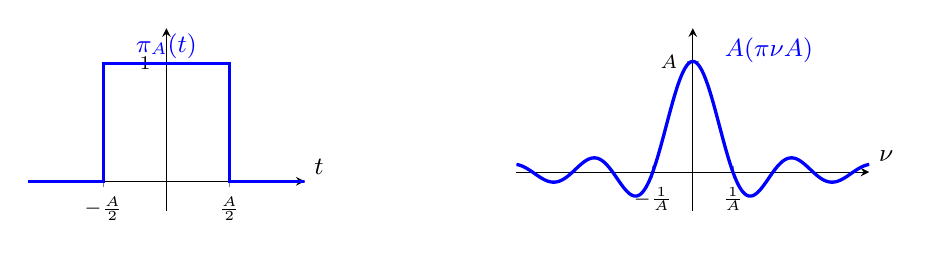
\begin{tikzpicture}
    \begin{axis}[
      width=0.42\textwidth, height=3.9cm,
      axis lines=middle, xmin=-1.1, xmax=1.1, ymin=-0.25, ymax=1.3,
      xtick={-0.5,0.5}, xticklabels={$-\frac{A}{2}$,$\frac{A}{2}$},
      ytick={1}, xlabel={$t$}, tick label style={font=\scriptsize},
      every axis x label/.style={at={(axis description cs:1.0,0.24)},anchor=west,font=\small},
      ]
      \addplot[blue,very thick] coordinates
        {(-1.1,0)(-0.5,0)(-0.5,1)(0.5,1)(0.5,0)(1.1,0)};
      \node[font=\small,blue] at (axis cs:0,1.15) {$\boldsymbol{\pi}_A(t)$};
    \end{axis}
    \begin{scope}[xshift=6.2cm]
    \begin{axis}[
      width=0.50\textwidth, height=3.9cm,
      axis lines=middle, xmin=-4.4, xmax=4.4, ymin=-0.35, ymax=1.3,
      xtick={-1,1}, xticklabels={$-\frac{1}{A}$,$\frac{1}{A}$},
      ytick={1}, yticklabels={$A$}, xlabel={$\nu$},
      tick label style={font=\scriptsize},
      every axis x label/.style={at={(axis description cs:1.0,0.30)},anchor=west,font=\small},
      ]
      \addplot[blue,very thick,domain=-4.4:4.4,samples=400]
        {sin(deg(pi*x))/(pi*x)};
      \node[font=\small,blue] at (axis cs:1.9,1.1) {$A\sinc(\pi\nu A)$};
    \end{axis}
    \end{scope}
  \end{tikzpicture}
  \caption*{\small A porte of total width $A$ and its transform, a cardinal
  sine of amplitude $A$ whose first zeros are at $\pm 1/A$. Narrowing the porte
  widens the sinc --- the changement d'échelle property.}
\end{figure}

\paragraph{Exemple intuitif : TF d'une fonction sinusoïdale infinie.} Si on
reprend le cas d'une onde plane monochromatique --- that of the first half of
the chapter --- au sens temporel du terme, représentable par un cosinus de durée
infinie, et si l'on se pose la question : « dans un cosinus $\cos(2\pi t/T_0)$
temporellement infini, combien y a-t-il de fréquences ? », l'étudiant répondra
naturellement qu'il n'y en a qu'une seule et qu'elle vaut $\nu=1/T_0$. Il aura
fait sans le savoir une transformée de Fourier :

\[
  V(t)=\cos\omega_0t=\cos 2\pi\nu_0t=\frac{1}{2}\left(e^{2j\pi\nu_0t}+e^{-2j\pi\nu_0t}\right)
  \ \xleftrightarrow{\ TF\ }\
  s(\nu)=\frac{1}{2}\left[\delta(\nu+\nu_0)+\delta(\nu-\nu_0)\right],
\]

où $\delta(\nu\pm\nu_0)$ représente une distribution de Dirac centrée en
$\mp\nu_0$. $s(\nu)$ est le spectre en amplitude, et

\[
  S(\nu)=|s(\nu)|^2
\]

est la \textbf{densité spectrale de puissance} (\textit{power spectral density})
de l'onde. Par définition, le \textbf{spectre électromagnétique}
(\textit{electromagnetic spectrum}) est la décomposition du rayonnement
électromagnétique selon ses différentes composantes en termes de fréquence ou
encore de longueur d'onde associée. Plus précisément, le spectre $S(\nu)$ est la
densité spectrale de puissance.

\begin{conclusion}
  Le spectre en amplitude d'une onde prenant la forme d'un cosinus de durée
  infinie est bien monochromatique, c'est-à-dire qu'il ne comprend qu'une et une
  seule fréquence (ou longueur d'onde).
\end{conclusion}

\begin{remark}[Fréquences négatives]
  La notion de fréquence négative n'a pas de réalité physique. Elles
  apparaissent lorsque l'on utilise les mathématiques pour comprendre la
  physique ! En effet, lorsque l'on développe $\cos 2\pi\nu_0t$ en exponentielles
  complexes, on voit apparaître des termes en $e^{2j\pi\nu_0t}$ et
  $e^{-2j\pi\nu_0t}$. On comprend à travers ces deux expressions que si
  $2\pi\nu_0$ est positif, alors, artificiellement, $-2\pi\nu_0$ devient
  négatif. Lors d'une interprétation physique, on n'oubliera pas de supprimer la
  partie négative du spectre : the two-line spectrum above is the
  \textbf{spectre mathématique} (\textit{mathematical spectrum}), the single
  line at $+\nu_0$ the \textbf{spectre physique} (\textit{physical spectrum}).
  Vu autrement, on peut aussi dire que pour un signal réel, nous aurons
  nécessairement $s(\nu)=s^{*}(-\nu)$ et que l'on peut donc se restreindre aux
  fréquences positives pour analyser complètement un signal puisque toute
  l'information y est contenue.
\end{remark}

\begin{notation}
  Dans les calculs, à partir de maintenant, on représentera une vibration par
  son signal analytique $V(t)$. Si les opérations sur $V(t)$ sont linéaires, on
  fera les calculs avec $V(t)$ puis on prendra la partie réelle $V_r(t)$ à la
  fin des calculs pour en déduire la vibration réelle et pouvoir ainsi faire une
  interprétation physique du phénomène observé. A general signal is then read
  as
  \[
    V(t)=\int_{-\infty}^{+\infty}\underbrace{s(\nu)}_{\text{amplitude of each component}\,\equiv\,\text{spectrum}}
      \underbrace{e^{2j\pi\nu t}}_{\text{term oscillating at }\nu\ \equiv\ \text{plane wave}}d\nu .
  \]
\end{notation}

\paragraph{Distribution de Dirac.}

\begin{definition}[Distribution de Dirac (\textit{Dirac distribution})]
  La distribution de Dirac $\delta(t)$ peut être définie comme une porte dont la
  largeur tendrait vers 0 tandis que sa hauteur tendrait vers l'infini de telle
  sorte que son aire, que l'on appelle également son \textbf{poids}
  (\textit{weight}), reste égale à $1$ :
  \[
    \delta(t)=\lim_{\varepsilon\to 0}\frac{1}{\varepsilon}\boldsymbol{\pi}_\varepsilon(t)
             =\lim_{\varepsilon\to 0}\frac{1}{\varepsilon}\boldsymbol{\pi}\!\left(\frac{t}{\varepsilon}\right).
  \]
\end{definition}

Cet objet mathématique représente en optique un point lumineux de taille
négligeable dans le domaine spatial, une impulsion de lumière infiniment courte
dans le domaine temporel ou encore une émission parfaitement monochromatique dans
le domaine spectral. Le Dirac revêt un aspect purement théorique et n'a pas de
sens physique on its own: un trou infiniment fin ne laisse pas passer de
lumière ! En optique, de surcroît, lorsque l'on fait tendre une porte vers une
largeur nulle, sa transmittance ne tend pas vers l'infini mais garde la même
valeur ! Ceci dit, lorsqu'on \emph{convolue} un Dirac avec une fonction,
c'est-à-dire en accord avec les lois de la physique (dérivable à dérivée
continue), le résultat est physique. La convolution sera abordée au chapitre
suivant.\\

Si on calcule la transformée de Fourier, en accord avec la propriété de
changement d'échelle, son extension étant temporellement nulle, l'amplitude de
son spectre sera au contraire infiniment étalée spectralement :

\[
  \delta(t)\ \xleftrightarrow{\ TF\ }\ \mathbf{1}(\nu),
  \qquad\qquad
  TF[\delta(t-\tau)]=\underbrace{e^{-2j\pi\nu\tau}}_{\text{dephasing}} .
\]

\begin{remark}
  The sign of the second relation is the one the translation property,
  $TF[f(t-\tau)]=e^{-2i\pi\nu\tau}F[\nu]$, and the appendix entry
  $\delta(\xi-\xi_0)\lra\exp(-2j\pi\xi_0\Xi)$ both give. A translation is a
  pure dephasing, of unit modulus, but its sign matters as soon as two such terms
  interfere.
\end{remark}

\begin{remark}
  On n'oubliera pas la flèche sur le Dirac quand on le représente sur un
  graphe. Cela montre qu'on ne représente pas son amplitude (qui est infinie)
  mais son aire (ou son poids).
\end{remark}

\paragraph{Distribution peigne de Dirac.}

\begin{definition}[Peigne de Dirac (\textit{Dirac comb})]
  Un ensemble d'impulsions de Dirac régulièrement espacées, d'expression
  analytique :
  \[
    \boldsymbol{\omega}_\tau(t)=\sum_{n=-\infty}^{+\infty}\delta(t-n\tau).
  \]
\end{definition}

On verra dans le chapitre suivant que l'on utilise souvent cette distribution
dans le cas de fonctions périodiques mais qu'elle n'a pas plus de sens physique
qu'un Dirac seul. On montre que le spectre d'un peigne de Dirac est également un
peigne de Dirac dont le pas a changé :

\[
  \boldsymbol{\omega}_\tau(t)=\sum_{n=-\infty}^{+\infty}\delta(t-n\tau)
  \ \xleftrightarrow{\ TF\ }\
  \frac{1}{\tau}\,\boldsymbol{\omega}_{1/\tau}(\nu)
  =\frac{1}{\tau}\sum_{n=-\infty}^{+\infty}\delta\!\left(\nu-\frac{n}{\tau}\right).
\]

\begin{remark}
  Le terme en $1/\tau$ devant les Diracs dans le domaine de Fourier peut être
  interprété comme un terme de conservation de l'énergie pour satisfaire au
  théorème de Parseval-Plancherel. It is the factor most often dropped. Beware
  also of mixing letters when transcribing from the appendix table, which names
  the step $L$ and the frequency $\Xi$: for the peigne de Dirac above the
  prefactor is $1/\tau$ and the teeth are $\delta(\nu-n/\tau)$.
\end{remark}

\begin{figure}[h!]
  \centering
  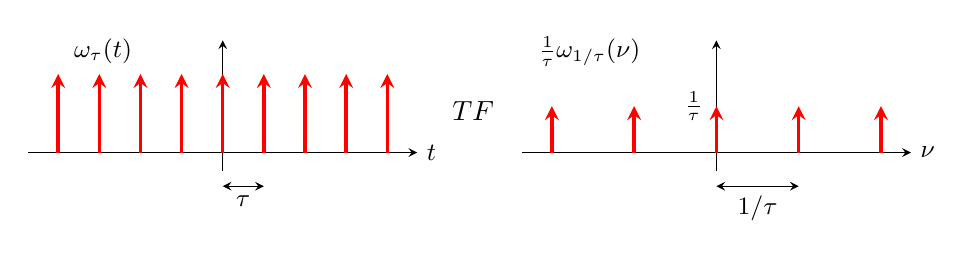
\begin{tikzpicture}[>=stealth,scale=0.95]
    \draw[->] (-2.6,0) -- (2.6,0) node[right,font=\small] {$t$};
    \draw[->] (0,-0.25) -- (0,1.5);
    \foreach \n in {-4,-3,-2,-1,0,1,2,3,4}{
      \draw[->,red,very thick] (\n*0.55,0) -- (\n*0.55,1.05);}
    \node[font=\small] at (-1.6,1.35) {$\boldsymbol{\omega}_\tau(t)$};
    \draw[<->] (0,-0.45) -- (0.55,-0.45) node[midway,below,font=\small] {$\tau$};
    \node at (3.35,0.55) {$\xleftrightarrow{\ TF\ }$};
    \begin{scope}[xshift=6.6cm]
      \draw[->] (-2.6,0) -- (2.6,0) node[right,font=\small] {$\nu$};
      \draw[->] (0,-0.25) -- (0,1.5);
      \foreach \n in {-2,-1,0,1,2}{
        \draw[->,red,very thick] (\n*1.1,0) -- (\n*1.1,0.62);}
      \node[font=\small] at (-1.7,1.35) {$\frac{1}{\tau}\boldsymbol{\omega}_{1/\tau}(\nu)$};
      \draw[<->] (0,-0.45) -- (1.1,-0.45) node[midway,below,font=\small] {$1/\tau$};
      \node[left,font=\small] at (-0.05,0.62) {$\frac{1}{\tau}$};
    \end{scope}
  \end{tikzpicture}
  \caption*{\small A peigne de Dirac of step $\tau$ and unit poids transforms
  into a peigne of step $1/\tau$ and poids $1/\tau$: tighten the teeth in time
  and they spread in frequency.}
\end{figure}

\subsubsection{Conséquence d'une troncature temporelle d'une onde monochromatique sur son spectre}

Si une vibration temporellement infinie correspond à un spectre monochromatique
par transformée de Fourier, il n'y a aucune raison pour qu'en \emph{tronquant}
temporellement cette onde lumineuse, sa TF reste une distribution de Dirac !\\

Or, le processus d'émission de lumière fait que les atomes n'émettent que
pendant un temps limité $\tau$, qui correspond à la durée de vie des états
excités dans la théorie quantique et au coefficient d'amortissement dans la
théorie classique. Une onde n'est donc jamais infinie temporellement !

\begin{conclusion}
  La conséquence d'une troncature temporelle d'une onde due au processus
  d'émission de la lumière est donc que son spectre n'est plus monochromatique.
  Il contient d'autres fréquences que la fréquence centrale. En pratique, c'est
  plus ou moins le cas suivant le type de source mais c'est toujours le cas.
  \textbf{Il n'existe pas de source parfaitement monochromatique} !
  Inversement, la conséquence du fait qu'une source ne soit jamais purement
  monochromatique est que les trains d'onde n'ont jamais une durée (ou une
  longueur) infinie.
\end{conclusion}

\subsection{Formules de Fresnel}

A complement, not developed in the rest of this chapter, whose conclusion is
used in the fibre chapter. For an onde incident at angle $i$ on a dioptre
between indices $n_1$ and $n_2$, refracted at $i'$, the amplitude reflection and
transmission coefficients split by polarisation --- $\parallel$ for the field in
the plane of incidence, $\perp$ for the field normal to it:

\[
  r_{\parallel}=-\frac{\tan(i-i')}{\tan(i+i')},\qquad
  t_{\parallel}=\frac{2\cos i\,\sin i'}{\sin(i+i')\cos(i-i')},\qquad
  r_{\perp}=-\frac{\sin(i-i')}{\sin(i+i')},\qquad
  t_{\perp}=\frac{2\cos i\,\sin i'}{\sin(i+i')} .
\]

\begin{conclusion}
  Le déphasage à la réflexion est $\pi$ (signe (-)) tant que l'on ne se trouve
  pas en réflexion totale. Dans le cas de la réflexion totale, ce déphasage est
  beaucoup plus compliqué et dépend à la fois de la polarisation et de l'angle
  d'incidence. Phénomène important dans la fibre optique !
\end{conclusion}
